%& C:\Users\Daniel\AppData\Roaming\TikzEdt\TikzEdt\023~1.0\TEMP_H~1
\begin{document}
\tikzset{zxgreen/.style={shape=circle,thick,draw,fill=green}}
\tikzset{zxred/.style={shape=circle,draw,thick,fill=red}}
\tikzset{zxyellow/.style={shape=rectangle,draw,thick,fill=yellow}}
\tikzset{zxdiamond/.style={shape=diamond,fill=black,inner sep=2.75}}
\tikzset{zxopen/.style={shape=circle,draw,thick,inner sep=2pt}}
\tikzset{->-/.style={decoration={markings,mark=at position .5 with {\arrow{>}}},postaction={decorate}}}
\tikzset{->-pos/.style={decoration={markings,mark=at position #1 with {\arrow{>}}},postaction={decorate}}}
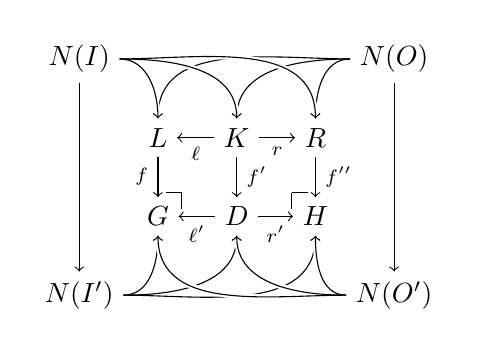
\begin{tikzpicture}

% middle stuff
\node (v1) at (0,0) {$L$};
\node (v3) at (1,0) {$K$};
\node (v5) at (2,0) {$R$};
\node (v6) at (0,-1) {$G$};
\node (v7) at (1,-1) {$D$};
\node (v13) at (2,-1) {$H$};
\draw [->] (v7) edge
	node [below] {\scriptsize $r'$}
	(v13);
\draw [->] (v5) edge
	node [right] {\scriptsize $f''$}
	(v13);

% top interface
\node (v2) at (-1,1) {$N(I)$};
\node (v4) at (3,1) {$N(O)$};
\draw [->] (v4) edge [out=180,in=90] (v1);
\draw [->] (v4) edge [out=180,in=90] (v3);
\draw [->] (v4) edge [out=180,in=90] (v5);
\draw [line width=1.75pt,white] (v2) edge [out=0,in=90] (v1);
\draw [line width=2pt,white] (v2) edge [out=0,in=90] (v3);
\draw [line width=2pt,white] (v2) edge [out=0,in=90] (v5);
\draw [->] (v2) edge [out=0,in=90] (v1);
\draw [->] (v2) edge [out=0,in=90] (v3);
\draw [->] (v2) edge [out=0,in=90] (v5);
\draw [->]  
	(v3) edge 
	node [below,pos=0.5] {\scriptsize $\ell$} 
	(v1);
\draw [->] 
	(v3) edge 
	node [below,pos=0.5] {\scriptsize $r$} 
	(v5);
\draw [->] (v1) edge
	node [left,pos=0.5] {\scriptsize $f$} 
	(v6);
\draw [->] (v3) edge 
	node [right,pos=0.5] {\scriptsize $f'$} 
	(v7);
\draw [->] (v7) edge 
	node [below,pos=0.5] {\scriptsize $\ell'$} 
	(v6);
	
% left corner
\node (v8) at (0.1,-0.7) {};
\node (v9) at (0.3,-0.7) {};
\node (v10) at (0.3,-0.9) {};
\draw  (v8.center) edge (v9.center);
\draw  (v9.center) edge (v10.center);

% right corner
\node (v15) at (1.9,-0.7) {};
\node (v14) at (1.7,-0.7) {};
\node (v16) at (1.7,-0.9) {};
\draw  (v14.center) edge (v15.center);
\draw  (v14.center) edge (v16.center);

% bottom interface
\node (v11) at (-1,-2) {$N(I')$};
\node (v12) at (3,-2) {$N(O')$};
\draw [->] (v11) edge [out=0,in=-90] (v6);
\draw [->] (v11) edge [out=0,in=-90] (v7);
\draw [->] (v11) edge [out=0,in=-90] (v13);
\draw [line width=2pt,white] (v12) edge [out=180,in=-90] (v7);
\draw [line width=2pt,white] (v12) edge [out=180,in=-90] (v6);
\draw [line width=2pt,white] (v12) edge [out=180,in=-90] (v13);
\draw [->] (v12) edge [out=180,in=-90] (v7);
\draw [->] (v12) edge [out=180,in=-90] (v6);
\draw [->]  (v12) edge [out=180,in=-90] (v13);
\draw [->] (v2) edge (v11);
\draw [->] (v4) edge (v12);



\usetikzlibrary{calc}
\pgftransformreset
\node[inner sep=0pt,outer sep=0pt,minimum size=0pt,line width=0pt,text width=0pt,text height=0pt] at (current bounding box) {};
%add border to avoid cropping by pdflibnet
\foreach \border in {0.1}
  \useasboundingbox (current bounding box.south west)+(-\border,-\border) rectangle (current bounding box.north east)+(\border,\border);
\newwrite\metadatafile
\immediate\openout\metadatafile=\jobname_BB.txt
\path
  let
    \p1=(current bounding box.south west),
    \p2=(current bounding box.north east)
  in
  node[inner sep=0pt,outer sep=0pt,minimum size=0pt,line width=0pt,text width=0pt,text height=0pt,draw=white] at (current bounding box) {
\immediate\write\metadatafile{\p1,\p2}
};
\immediate\closeout\metadatafile
\end{tikzpicture}

\end{document}


